%
% Florent JACQUET - Antonin Waltz
%
% Rapport de LO43 (A14)
%   SmallUTBMworld
%
%

\documentclass[a4paper]{report}

%packages
\usepackage[utf8]{inputenc}
\usepackage[francais]{babel}
\usepackage{graphicx}\graphicspath{{pictures/}}
\usepackage{float}
\usepackage[T1]{fontenc}
\usepackage{color}
\usepackage{fancyhdr}
\usepackage{listings}
\usepackage[colorlinks=true,allcolors=black]{hyperref}
\usepackage[font=small,labelfont=bf,margin=\parindent,tableposition=top]{caption}

\setcounter{tocdepth}{2}

\begin{document}

\begin{titlepage}
    
\includegraphics[width=0.4\textwidth]{logo_utbm.png}
    \begin{center}
        \textsc{\LARGE Université de Technologie de Belfort Montbéliard}\\[1cm]
        \textsc{\Large LO43}\\
        \rule{\linewidth}{0.5mm}
        { \huge \bfseries Smallworld UTBM\\[0.4cm] }
        \rule{\linewidth}{0.5mm}
        \vskip1cm
        % Author and supervisor
        Florent \textsc{Jacquet}\\
        Antonin \textsc{Waltz}\\
        Superviseur: Amine \textsc{Ahmed Benyahia}\\
        \vskip1cm
        %\includegraphics[width=0.6\textwidth]{smallworld.png}
        \vfill
        {\large Automne 2014}
    \end{center}
\end{titlepage}


\newpage
\tableofcontents
\listoffigures

\newpage
\chapter{Présentation du projet}
\par
Durant ce semestre en LO43, nous avons choisi le projet \textit{Smallworld}
parmi tout ceux proposés.
\par
\textit{Smallworld} est un jeu de stratégie qui propose de gérer la destinée de
peuples fantastiques, chacun disposant d'une particularité unique. En plus de
ça, ceux-ci sont associés aléatoirement à un pouvoir spécial qui leur confére
une capacité supplémentaire.
\par
Le but est de conquérir des territoires afin d'obtenir le plus de points de
victoire. Cependant au fur et à mesure de l'avancé du jeu, un peuple a tendance
à s'affaiblir.  Le joueur qui le contrôle peut alors le faire passer en déclin
et choisir une nouvelle civilisation.
\par
Nous avons adapter les peuples et les pouvoirs à l'environnement de l'école, en
respectant les régles de base du jeu.
%TODO à compléter

\newpage
\chapter{Organisation et répartition du travail}
\par
Notre groupe étant composé de 2 personnes, il était facile pour nous de
communiquer sur l'avancé du projet, la façon d'aborder telle ou telle contrainte
technique ou fonctionnelle ou tout simplement faire le point.
\par
Dans un premier temps et après nous être approprié \textit{Smallworld}, nous
avons réaliser les spécifications UML ensemble afin de partir sur la même base
de départ. Evidemment nous adapterons au fur et à mesure de l'implémentation en
fonction de l'évolution des contraintes. Nous nous sommes également mis d'accord
sur l'utilisation du pattern MVC, du polymorphisme, etc.
\par
Concernant les outils, nous avons utilisé \textbf{Eclipse}, \textbf{Dia} pour
l'UML et un dépôt \textbf{Git} pour la synchronisation des sources et le
versionnage. Nous avons également profiter des fonctionnalités de \textbf{Git}
pour effectuer un suivi efficace des fonctions à modifier où terminer.
\par
La répartition du travail s'est globalement fait ainsi, sachant que chacun
n'hésitait pas à intervenir dans les parties de l'autre si besoin était :
\begin{itemize}
    \item Florent : %TODO à compléter
    \item Antonin : %TODO à compléter
\end{itemize}

\newpage
\chapter{Architecture du projet}
\section{Premiere approche (Cas d'utilisation)}


\section{Le modele}


\section{L'interface (la Vue)}


\section{Le deroulement d'une phase de jeu (Sequence)}


\newpage
\chapter{Implementation}


\newpage
\chapter{Annexes}
\section{Diagramme de cas d'utilisation}
\begin{figure}
    \begin{center}
        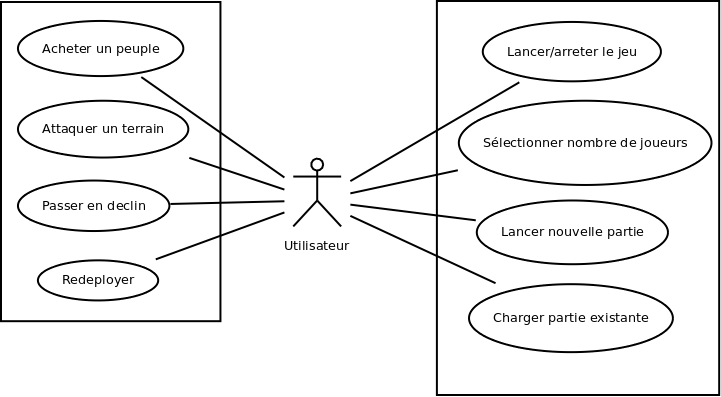
\includegraphics[width=\textwidth]{use_case.png}
        \caption{Diagramme des cas d'utilisation du \textit{Smallworld}}
    \end{center}
\end{figure}
\section{Diagramme de séquence}
\begin{figure}
    \begin{center}
        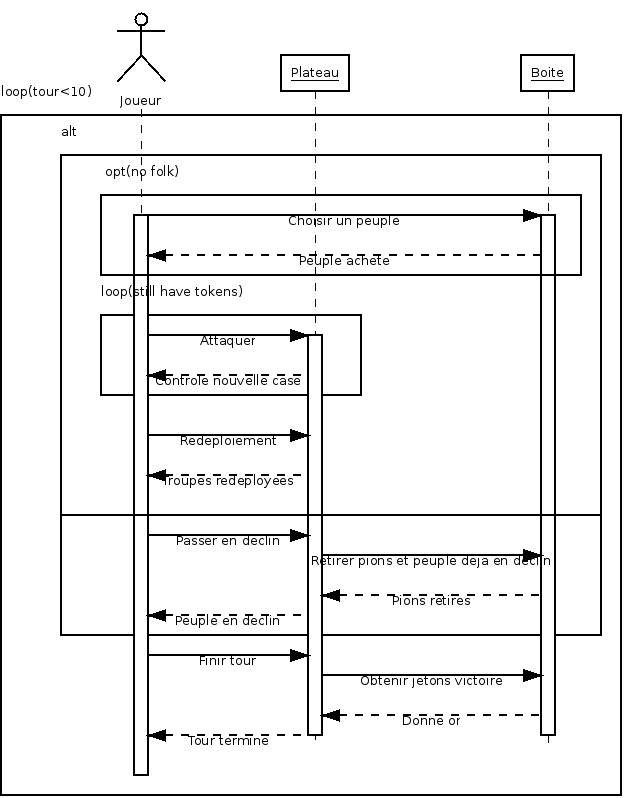
\includegraphics[width=\textwidth]{sequence.png}
        \caption{Diagramme de séquence d'un tour de jeu}
    \end{center}
\end{figure}
\section{Diagramme de classes}
\begin{figure}
    \begin{center}
        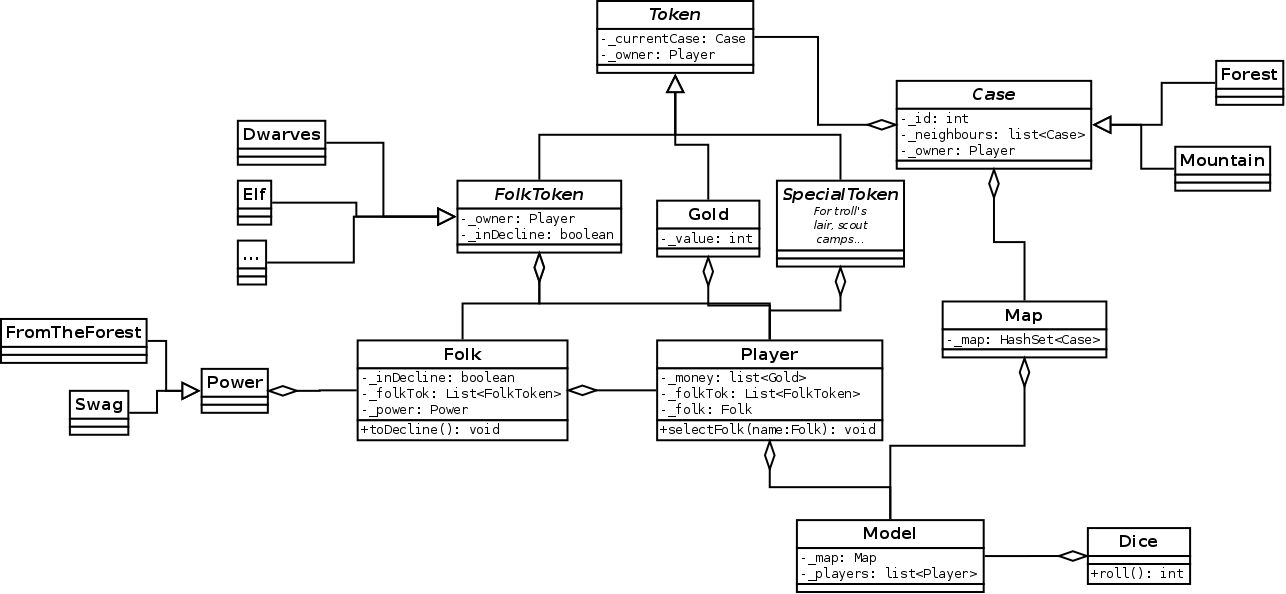
\includegraphics[width=\textheight,angle=90]{classe.png}
        \caption{Diagramme de classe du modèle}
    \end{center}
\end{figure}

\end{document}

